\documentclass[12pt]{article}
\usepackage[russian]{babel}
\usepackage[utf8x]{inputenc}
\usepackage{amssymb}
\usepackage{amsmath}
\usepackage{graphicx}
\usepackage{geometry}
\usepackage[colorinlistoftodos]{todonotes}
\usepackage{listings}
\usepackage[section]{placeins}
\begin{document}

\title{5. Оценивание характеристик стационарного случайного процесса}
\author{Андрей Валиков}
\date{}
\maketitle
																																																								\section{Формирование последовательности случайных чисел}
																																																	
\[N = 500\]  
	
	  
Параметры случайной функции:
\[a = 0.24\]
\[b = 2\]
\[r(n)= b * \textrm{rand}\]	


Вычисление последовательности:
\[x(n) = ( 1 − a ) ⋅ x(n − 1) + a ⋅ \nu(n), n = 1, 2, ..., N −1\]



\begin{lstlisting}
def RP(N, a, b):
  y = np.zeros(N)
  x = b * np.random.rand(N)
  y[0] = b / 2

  for n in range(1, N):
    y[n] = y[n - 1] * (1 - a) + a * x[n]

  return y
\end{lstlisting}

Получаем следующую гистограмму частоты встречаемости.
\begin{figure}[!htb]
\centering
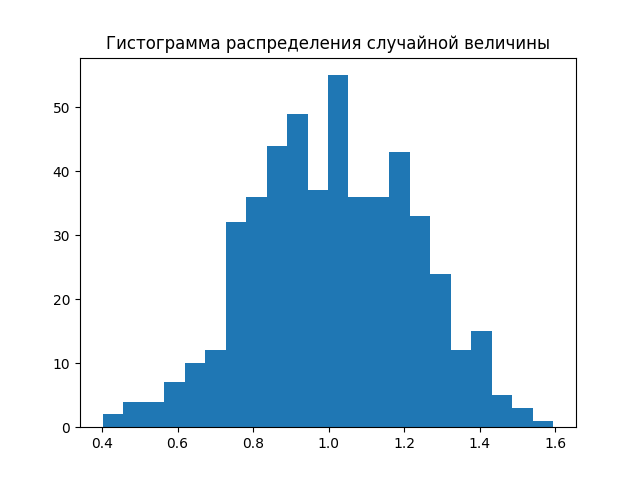
\includegraphics[scale=1.00]{hist.png}
\caption{}
\label{}
\end{figure}


\section{Характеристики случайной последовательности}
Математическое ожидание:

\[M(X) = \frac{1}{N}\sum_{n=0}^{N - 1}x(n)\]


\begin{lstlisting}
m = np.mean(x)
\end{lstlisting}

1.001

Дисперсия:
\[D(X) = \frac{1}{N - 1}\sum_{n=0}^{N - 1}(x(n) - M(X))^2\]
\begin{lstlisting}
d = np.mean((x - m) ** 2)
\end{lstlisting}

0.044
       

\section{Корреляционная функция}



\[R(m) = \frac{1}{N - m} \sum_{n=0}^{N - m - 1}(x(n) - M(X))(x(n+m) - M(x)) \]
Используем $M < \frac{N}{10}$

\begin{lstlisting}
def R(X, M):
  N = len(X)
  L = N // 10 - 1
  y2 = np.zeros(L)

  for m in range(L):
    for n in range(N - m):
      y2[m] += (X[n] - M) * (X[n + m] - M)
    y2[m] /= N - m

  y = np.append(np.flip(y2, axis=0), y2)
  return y
\end{lstlisting}


\begin{figure}[!htb]
\centering
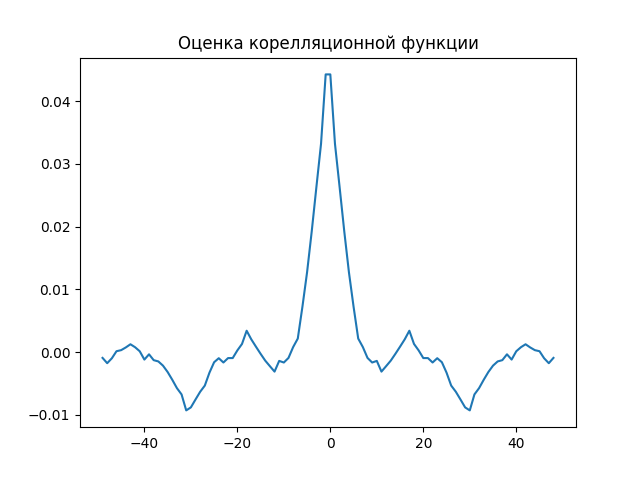
\includegraphics[scale=1.00]{corell.png}
\caption{}
\label{}

\end{figure}


\section{Вывод}
Рассматривались статистические характеристики случайных процессов, при помощи которых можно делать выводы о свойствах данных процессов или систем. В случае эргодичности случайного процесса, судить о его свойствах можно основываясь на одной его реализации. 
Получены следующие характеристики случайного процесса:\\
    • Оценка математического ожидания: 1.001;\\
    • Оценка дисперсии случайного процесса: 0.044;\\
    • Оценка корреляционной функции – Рисунок 2;\\
При изучении полученных характеристик реализации случайного процесса, а также построенной гистограмме, можно сделать вывод о том, что после использования цифрового фильтра – распределение случайного процесса больше не является равномерным, а большинство значений случайного процесса сконцентрированы в промежутке [0.8; 1.1].

\end{document}